% !TEX root = _yoko.tex

% ==========================================
% プロジェクト予稿（1P）の本文
% ==========================================

\section{はじめに}
音楽は，今日多くの人にとって日常の一部となっており，その楽しみ方も多岐にわたる．音楽は人々の感情や想いを表現し共有する手段の１つとなっている．本研究\cut{で}は，作品制作を通して\red{空間における音楽映像体験(?)}を提供することを目的とする．
%作品制作では，を誰もが再現できるような簡易的な素材と技術を用いて楽器の生演奏に合わせた空間演出を行う． 

\sectionmargin
\section{\red{制作方針}}
%音楽は様々な要素から成り立っており，演出表現を行う際に大きな役割を持つ．

\red{
    音楽を介して世界観が成立する要素として，「\emph{譜面的要素}」と「\emph{背景的要素}」に着目する．
}

\begin{description}
    \item[譜面的要素] 音高や音量の変化，コード進行による曲調の変化，楽器構成\red{を指す}．聴衆\red{の}感情や認知に影響をもたらすことが多く，歌詞や曲調を手掛かりとした照明演出に\red{利用されている}\cite{Kanno22}．
    \item[背景的要素] 曲の制作過程や，演奏者の想い，\red{作品}の主題歌であるかなど\red{を指す}．聴衆に具体的な情景を想起させるための手掛かりとなる．
\end{description}
%
これらの要素を踏まえ，福知山公立大学3201の教室を利用して，\red{３つ}の作品制作を行った．

\sectionmargin
\section{作品の世界観を再現する演出表現}
\red{映画「}アラジン\red{」}の主題歌「A Whole New World」\cite{Aladdin}\red{を通じて，作品の持つ世界観を，ピアノ演奏，映像，ステージ演出を通じて表現する試みを行った．}
%自身が演奏者として演奏しつつ，複数人での作品制作を行った．本作品においては，アラジンの主題歌として大変有名な楽曲であるため，アラジンの世界観を再現した空間を表現することを目的とした．

%本作品において意識・工夫した点は，映像のみではなく，空間でアラジンの世界観を表現する点である．
\red{演奏は}ピアノ初心者\red{である筆者が行った．}
\red{
    星の流れる映像をピアノのMIDI出力によって制御したり，ドライアイスや，ペットボトルを利用した簡易ライトをスクリーン前の床に配置して，雲や星空が立体的に表現されるようにした．
    映像の切替は協力者に手動で行ってもらうことで，演奏ミスやテンポに左右されない実演をすることができた．
}

\sectionmargin
\section{映像空間の拡張を目指した演出表現}
%2つ目の作品制作として
大塚愛「プラネタリウム」\cite{Planetarium}\red{のメロディや歌詞に焦点を当て，
    ピアノ演奏と楽曲の雰囲気に合わせた視覚演出の表現を行った}．
%
\red{具体的には，備付}のスクリーン\red{と}ピアノの側面\red{の２箇所に独立した}映像を投影させ\red{た（図\ref{fig:planet}）．}

\begin{description}
    \item[(1)ピアノ側面映像:] 歌詞と背景画像．楽曲の\red{譜面的要素である歌詞に基づき，「}星空や夜景\red{」}を表現する．\red{側面に映像投影をすることで，その奥でピアノを演奏する奏者の動きと影も視界に入る．これにより，直接的な譜面的要素の視覚演出に繋げていく．}
    \item[(2)スクリーン映像:] 夕暮れから夜にかけての風景．楽曲の\red{背景的要素である「}夏の幻想的で切ない様子\red{」}を表現する．\red{さらに}，演奏者の映像を複数カメラで撮影し，映像と合成することで\red{，}\red{演奏者も際立てる???ようにした}．
\end{description}


\red{これにより，}
聴衆の視点\red{が，}演奏者\red{，ピアノ本体，スクリーンを往来し，演奏空間を多角的に観ることができるようにした．}


\begin{figure}[tb]
    \centering
    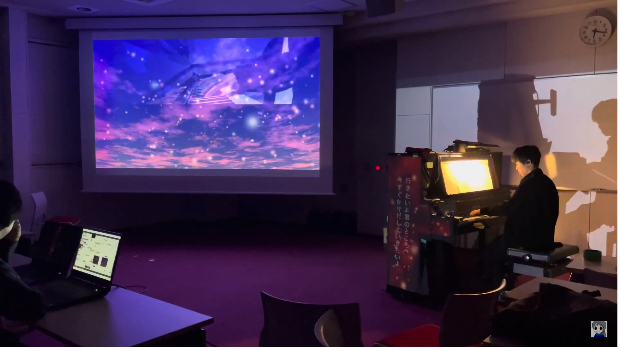
\includegraphics[width=\linewidth]{fig/fig5-planet-play}
    \caption{作品発表の様子}
    \label{fig:planet}
\end{figure}

\section{演奏者の魅力を引き出す演出表現}
%3つ目の作品として
YOASOBIの「ラブレター」\cite{loveletter}\red{を題材とし，}トランペットとエレキギターの生演奏に合わせて部屋の壁一面を投影\red{する}演出表現を行った．

本作品では音楽が大好きな演奏者2人の気持ちを表現するような演出を施し，最後には両端に演奏者が大きく映し出されるようになっている．また，生成AIを使用することで，より幅広く細かな表現を施すことができた．今後はより演奏者の動きや演奏に合わせた演出や，生演奏であることにこだわった見せ方をしたいと考えている．

\section{考察}
本研究を通してもっとも重要だった点は，演出表現を行うにあたって聴衆に最も魅せたいものは音楽のどの要素であるかを明確にする点である．譜面的要素の場合は，テンポや音色に合わせた色の変化や図形やイラストの動きといった視覚表現が多用される．一方で背景的要素に注目する場合は，具体的な物を視覚化することで観客にストレートな表現ができる．一方で演奏者やストーリーに注目させたい場合は図や色のみを用いた抽象的表現により観客に楽曲の世界を創造させ新たな魅力を発見させるきっかけとなる．

\section{おわりに}
本研究では，身近な素材と技術を用いた作品制作を通して，空間における音楽映像体験を提供することを目的とした．今後はより空間全体を意識し，観客の視線誘導や演奏の自由度や，演奏者の動きを考慮した作品制作を行っていきたいと考える．

\vspace{12pt}
\small